\subsection{Red Laboratorios DC}

Para este experimento, capturamos los paquetes de la LAN Wi-Fi Laboratorios-DC del Departamento de Computació de la FCEyN de la UBA. La medición fue realizada un día Lunes desde las 15hs y durante 15 minutos. La cantidad de paquetes capturados es de 4000. De estos, 164 corresponden al protocolo ARP.

\begin{figure}[H]
       \centering
       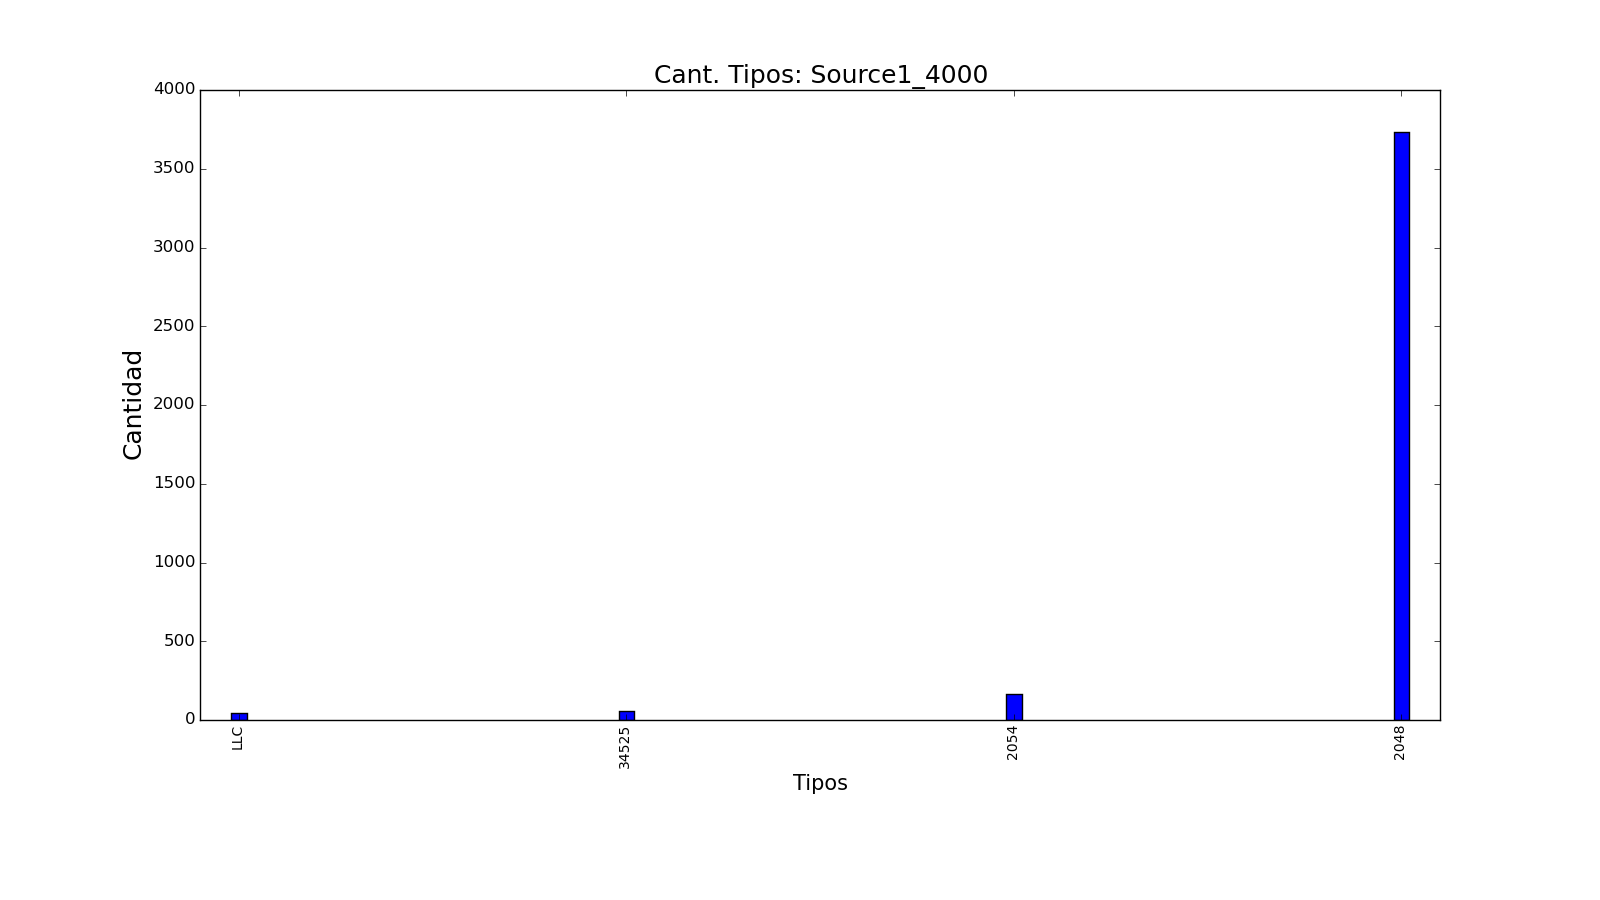
\includegraphics[width=1\textwidth]{../resultados/labo-corrida3/histogram_types.png}
       \caption{Protocolos de los paquetes capturados}
       \label{red-Starbucks-types}
\end{figure}

En este caso, el overhead impuesto por los paquetes ARP es de 4.1\%.

\begin{figure}[H]
       \centering
       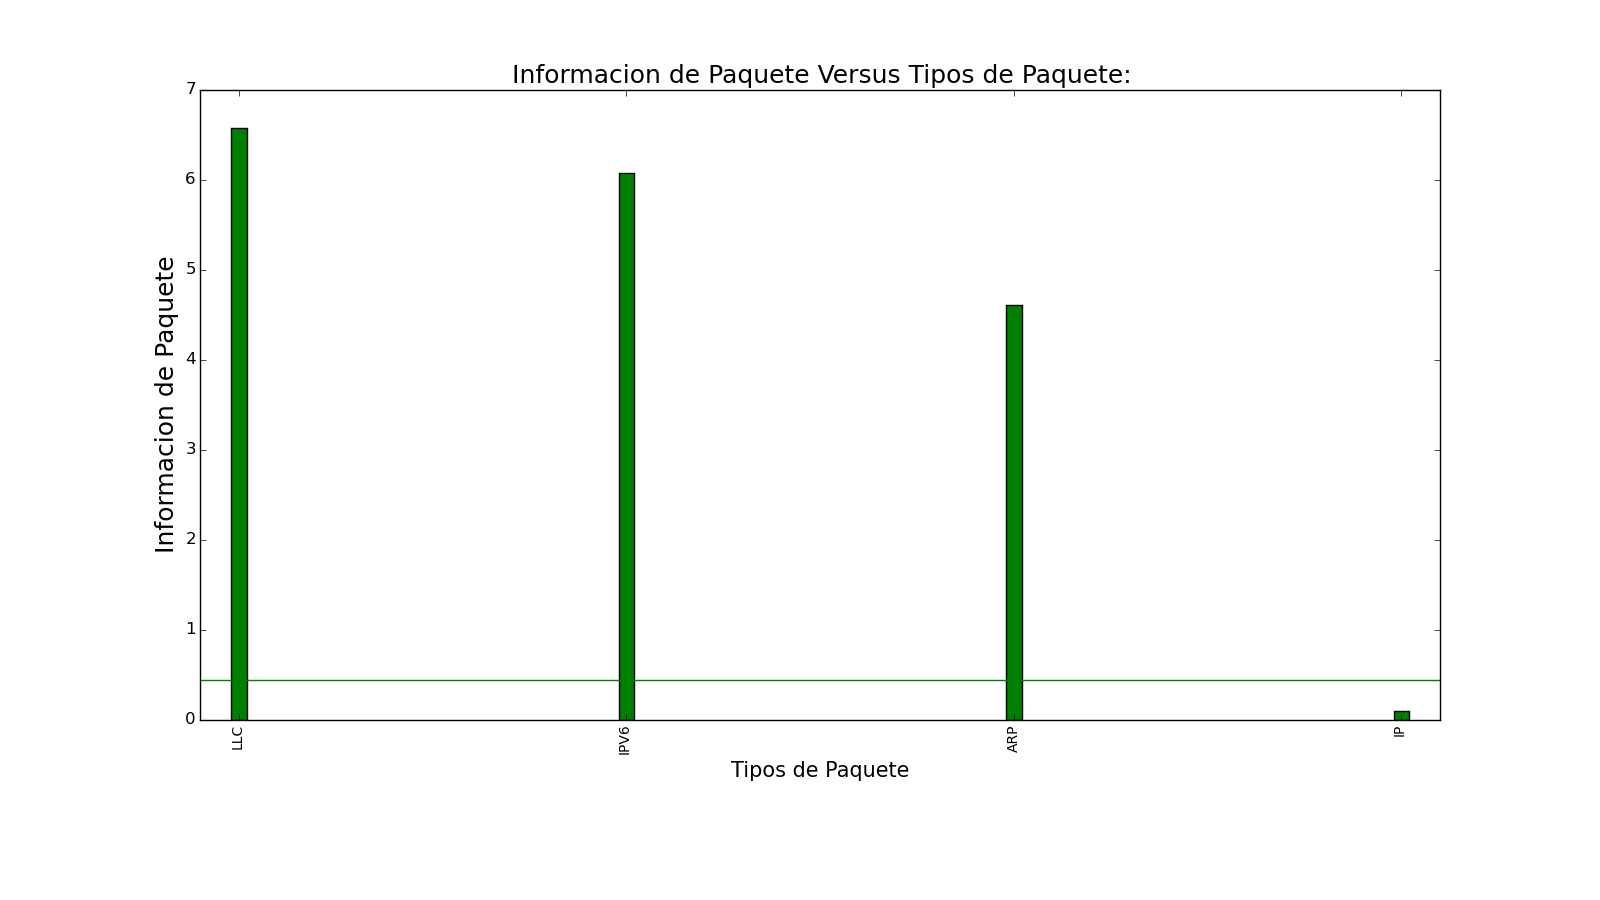
\includegraphics[width=1\textwidth]{../resultados/labo-corrida3/histogram_types_information.png}
       \caption{Información de los protocolos de los paquetes capturados}
       \label{red-Starbucks-types-information}
\end{figure}

Como podemos observar también en este experimento, de acuerdo a nuestra definición de protocolo distinguido, el protocolo IPv4 sería el único distinguido en esta fuente. Es razonable, ya que la cantidad de paquetes IPv4 es mucho mayor que la cantidad de paquetes IPv6, LLC y ARP. La información de los paquetes IPv4 es \textbf{0.0988917569855}, mientras que la entropía de la fuente es \textbf{0.440025436837}. Se observa como la información es claramente menor a la entropía.

\begin{figure}[H]
       \centering
       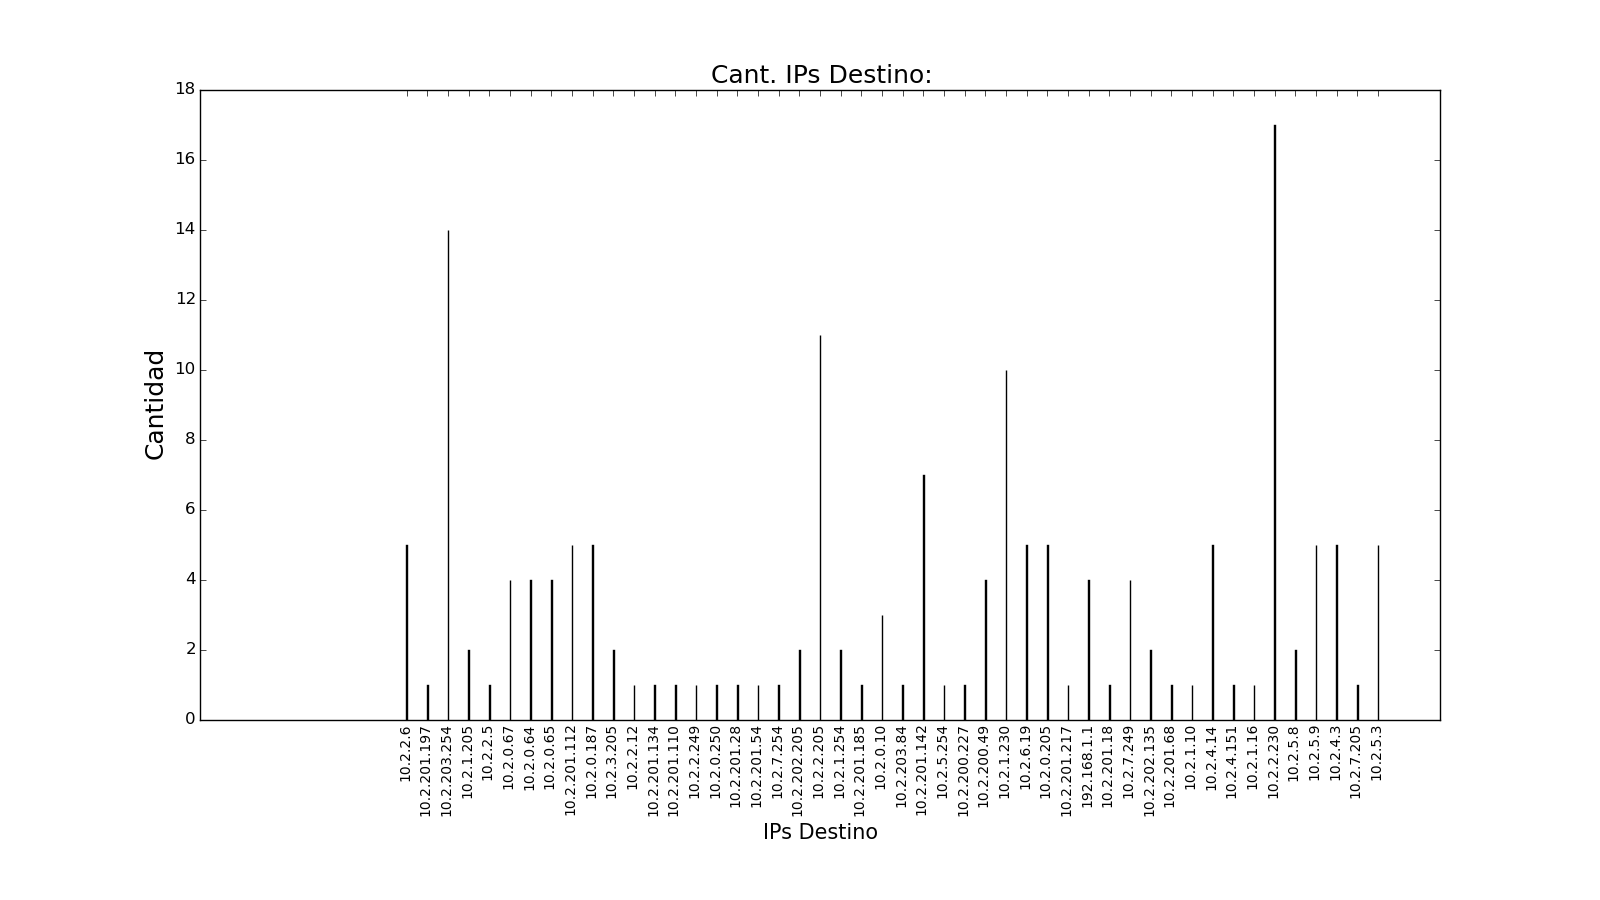
\includegraphics[width=1\textwidth]{../resultados/labo-corrida3/histogram_dst.png}
       \caption{IPs destino de los paquetes ARP}
       \label{red-Starbucks-dst}
\end{figure}

\begin{figure}[H]
       \centering
       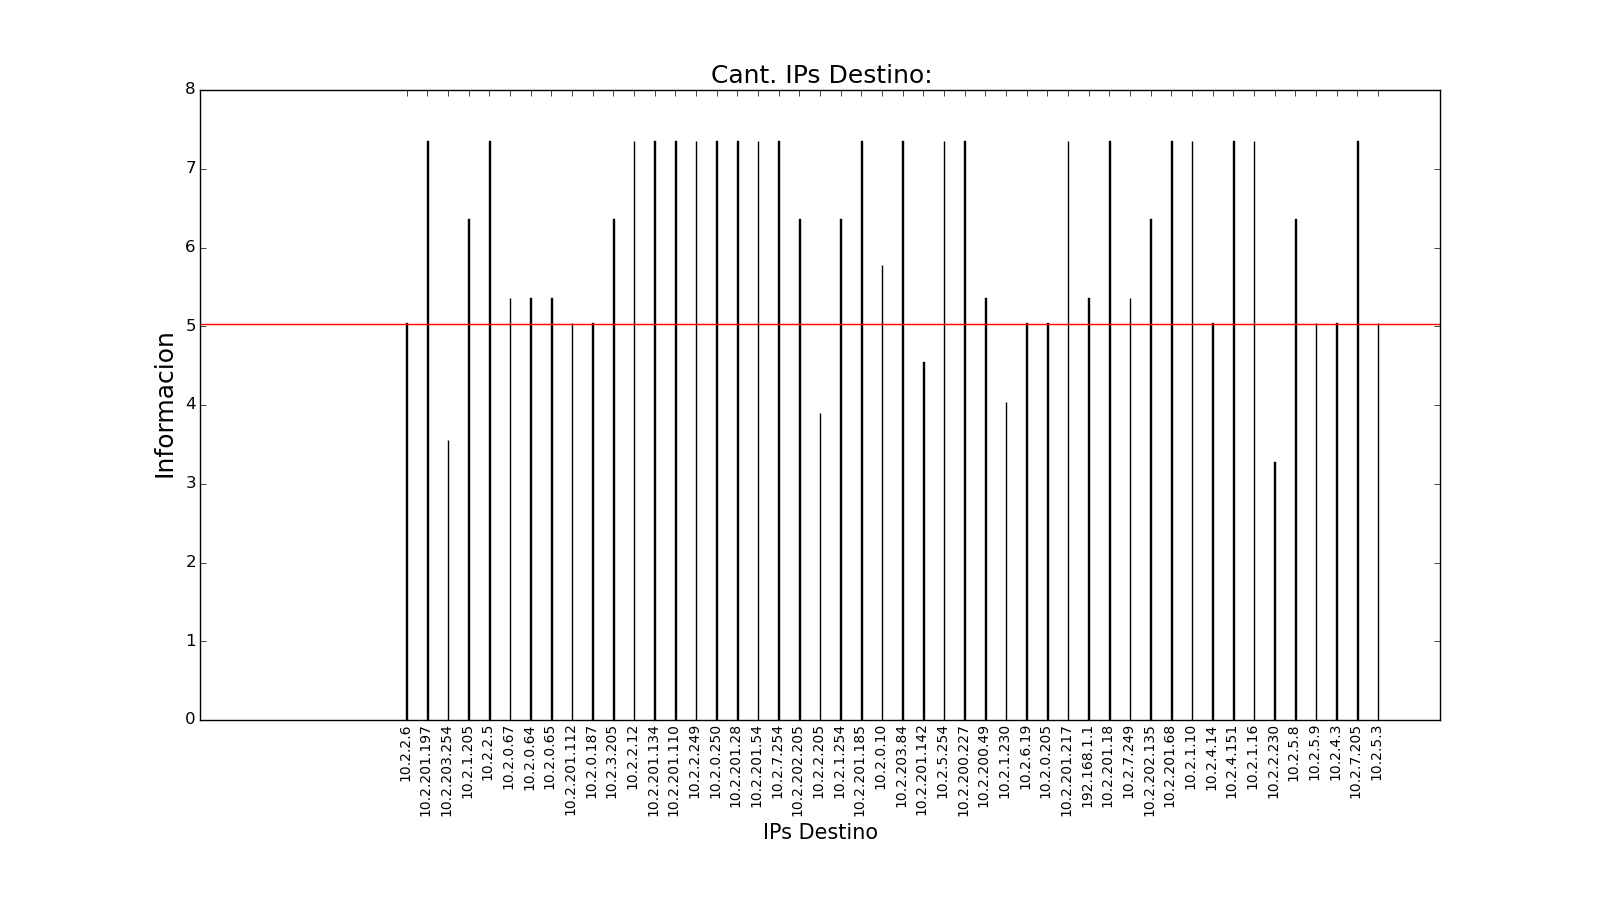
\includegraphics[width=1\textwidth]{../resultados/labo-corrida3/histogram_dst_information.png}
       \caption{Información de IPs destino de los paquetes ARP}
       \label{red-Starbucks-dst-information}
\end{figure}


\begin{figure}[H]
       \centering
       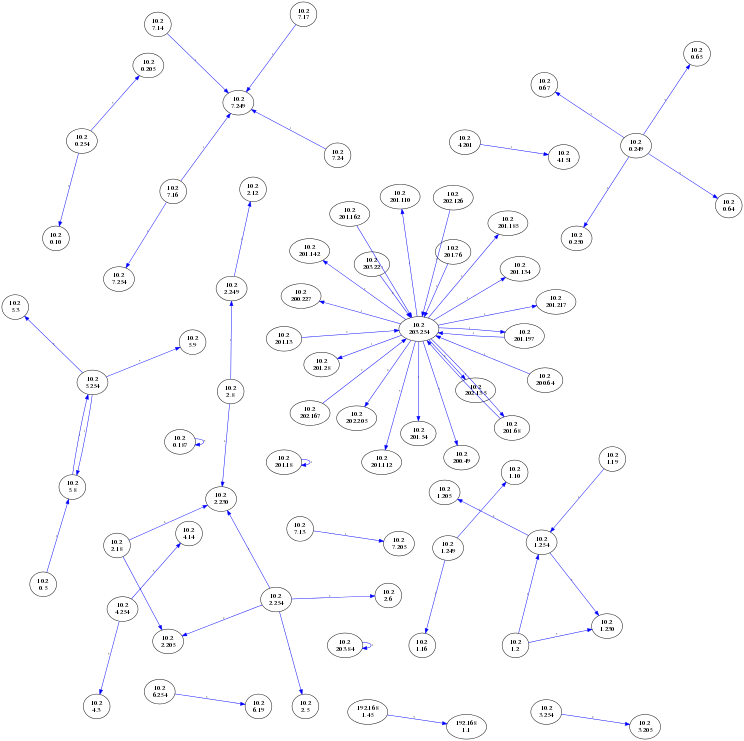
\includegraphics[width=1\textwidth]{../resultados/labo-corrida3/network.png}
       \caption{Tráfico de paquetes ARP}
       \label{red-Starbucks-dst-information}
\end{figure}

Analizando la información de estos gráficos vemos como la IP \textbf{10.2.203.254} parece ser el router: recibe una mayor cantidad de paquetes que casi todas las demás IPs, es un nodo distinguido por ser su información menor a la entropía, y las conexiones que tiene son a las IPs 10.2.200.X, 10.2.201.X y 10.2.202.X, que deben ser subnets.\\

También vemos por ejemplo que la IP \textbf{10.2.2.230} recibe incluso una mayor cantidad de paquetes y  también es un nodo distinguido, pero esa mayor cantidad de paquetes viene desde pocos nodos. Creemos por esto que puede tratarse de algún servidor (de datos, de imágenes, etcétera).
